%%
%% Capítulo 4: Desenvolvimento
%%

\mychapter{Desenvolvimento}
\label{Cap:Desenvolvimento}

O principal objetivo desse trabalho é criar um controlador para
um Andador inteligente, sendo este controlador pensado para requerer
pouca memória e processamento, também visa-se estudar e aplicar algoritmos
de aprendizagem de máquina de modo a gerar um modelo cinemático do robô.
O modelo cinemático é o maior desafio deste trabalho, pois como será visto
mais adiante foi utilizado uma abordagem que mescla a solução analítica com
algoritmos de aprendizado de máquina para gerar um modelo de um robô com
acionamento diferencial, outra contribuição deste trabalho é o modelo do
robô simulado, onde o controlador, e o modelo cinemático foram avaliados.
O desenvolvimento do controlador, foi dividindo em quatro partes, a primeira
é a construção da simulação do robô, segunda foi a coleta de dados para
a construção do modelo cinemático, terceira foi  modelado
uma rede neural de modo que seus parâmetros se traduzissem nos parâmetros
da cinemática, quarta e ultima parte conta o desenvolvimento
do pre-processamento dos dados. 


\section{construção do robô em um ambiente simulado}
O simulador utilizado para a construção do robô foi o CoppeliaSim
\cite{rooban2021coppeliasim}, antigamente conhecido como V-REP.
Uma das contrições deste trabalho foi a criação de um cliente 
\textit{zmqRemoteApi} para a linguagem de programação \textit{Rust}
que se comunica com o simulador, \textit{Rust} foi adotado pois
é capaz de produzir um código tão performático quando C/C++, além
de possui um gerenciador de pacotes que facilita o desenvolvimento
futuro de novas aplicações e reutilização de códigos. O ambiente
simulado possui o formato quadro com um lado $l$ de 5 metros,
além do robô, o ambiente possui um alvo, a qual o robô deve-se ir
atrás dele, o alvo é um objeto que pode ser movido com mouse. 

\begin{figure}[H]
    \centering
    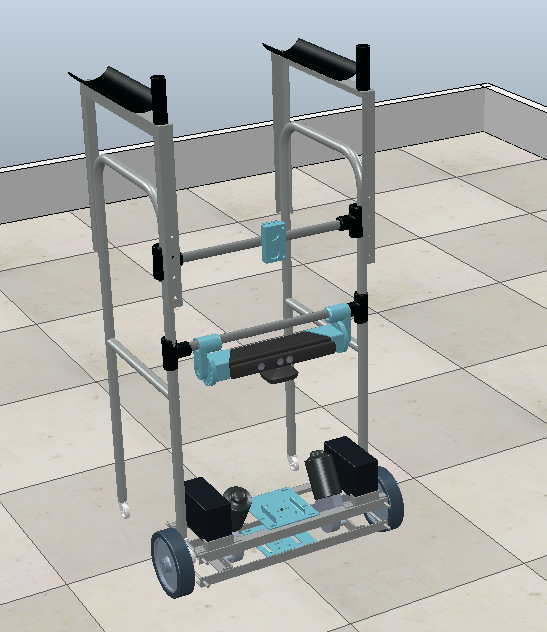
\includegraphics[scale=0.2]{figuras/robo_simulado_1.png}%
    \hspace{1cm}
    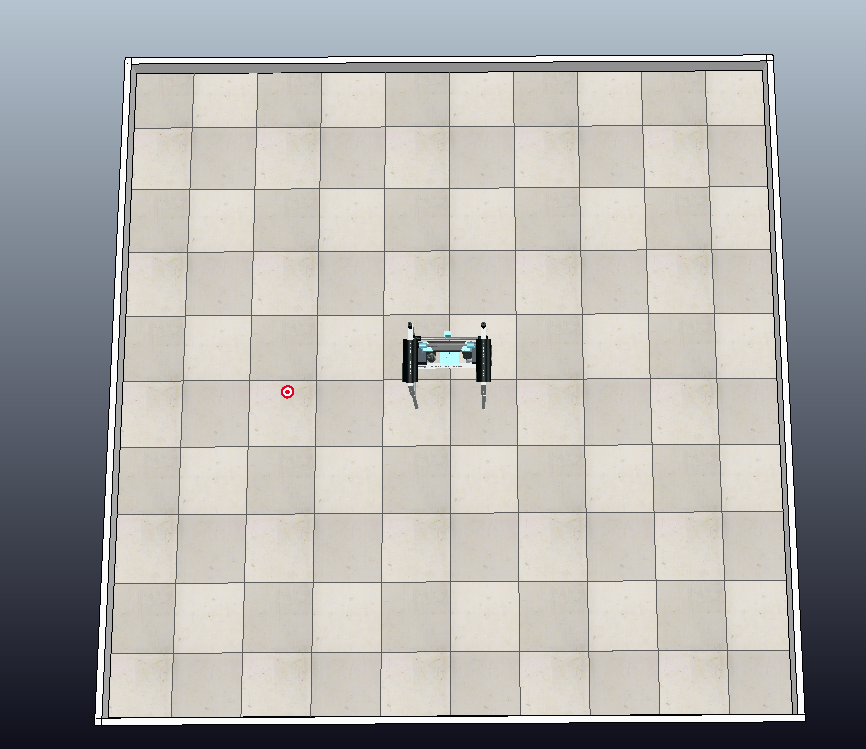
\includegraphics[scale=0.2]{figuras/visao_cima.png}
    \caption{Andador inteligente simulado}
\end{figure}

Como dito anteriormente, o robô possui um acionamento diferencial,
o CoppeliaSim, permite configurar os atuadores no modo controle de
velocidade, neste modo, o cliente \textit{zmqRemoteApi} é capaz de enviar
um sinal em radianos por segundo, a qual é aplicado instantaneamente.
O modelo conta com sensores para odométrica como giroscópio e acelerômetro
e um kinect, no entanto os sensores não foram utilizados neste trabalho,
foi utilizado funções do próprio simulador para coletar posição e 
orientação do robô em relação ao referencial global.

\section{Coleta de dados para o modelo cinemático}
Tendo o robô modelado, a simulação configurada, então foi criado
um algoritmo que faça o robô andar aleatoriamente pelo cenário ao mesmo
tempo que se coletava a posição e orientação do robô em relação ao referencial
global. O pseudo código pode ser observado no Algoritmo \ref{coleta:de:dados:}

\begin{algorithm}[H]
    \label{coleta:de:dados:}
    
    \Entrada{$N_a$:número de amostras, $K$: número de paços continuos }
    %% \SetLine
    
    inicialize a conexão SIM  com o simulador

    inicialize a memória $M$

    mova o robô R para a origem e com uma orientação aleatória $\theta$,
    por meio da conexão SIM

    \Para {$e \leftarrow 0$ \Ate $N_a$} {
        leia a posição $x_1$,$y_1$  e orientação $\theta_{1}$ do robô,
        referente a origem, por meio da conexão SIM
        
        leia o tempo $t_1$ da simulação,por meio da conexão SIM
        
        gere as velocidades das rodas $\phi_l$,$\phi_r$ aleatoriamente,
        entre [0,$V_{MAX}$]
        
        envie  $\phi_l$,$\phi_r$, para o robô simulado pela conexão SIM

        permita que a simulação ocorra por 50ms 

        leia a posição $x_2$,$y_2$  e orientação $\theta_{2}$ do robô,
        referente a origem, por meio da conexão SIM

        leia o tempo $t_2$ da simulação.por meio da conexão SIM

            \Se {$e$ é múltiplo de $K$}{
                
                mova o robô R para a origem e com uma orientação aleatória $\theta$,
                por meio da conexão SIM
            }
        
        armazene em $M$ os valores  $(x_1,y_1,\theta_{1},t_1,\phi_l,\phi_r),(x_2,y_2,\theta_{2},t_2)$
        
    }

    armazene $M$ em um arquivo
    
    \caption{Algoritmo de Coleta de dados}
    
\end{algorithm}

O parâmetro $K$ do algoritmo foi criado para que o robô não bata na parede
da simulação, ele foi encontrado fazendo um teste empírico, mostrando que
após 20 paços  com o robô caminhando em linha reta, o robô bate na parede,
por tanto nos nossos testes $K = 18$. Um princípio foi adotado na coleta
de dados: o robô deve-se mover lentamente em todas a direções, sabendo do
fato que a velocidade linear máxima do robô é 0,8 metros por segundo,
por tanto foi adotado que velocidade linear máxima da coleta seria de 
0,165 metros por segundo, esse número foi adotado por ser significantemente,
inferior a 0,8  e ser o dobro do raio das rodas, ou seja, na prática é gerado
dois números aleatórios de distribuição uniforme entre 0 e 1 e multiplicado por
2, $V_{MAX} = 2$. O simulador retorna valores de posições $x$,$y$ em metros
que variam de -2,5 até 2,5 metros, já a orientação do robô é medida em radianos
que variam de $-\pi$ até $\pi$.

\section{Modelagem de parâmetros de redes neurais artificiais}
Atualmente \textit{Frameworks} de aprendizado máquina supervisionado,
tem evoluído bastante, uma das principais técnicas que revolucionou a
área de aprendizado de máquina é uma estrutura de dados chamada grafo
computacional, ele é o um grafo direcionado e acíclico de operações com
tensores, onde um nó pode ser um tensor ou uma função que opera sobre
tensores. A figura \ref{fig:grafo:computacional} é um exemplo de
grafo computacional que foi retirada do livro \cite{chollet2021deep},
onde $x$ e $y_{true}$ são as variáveis de entrada, e $w$ $b$ são
os parâmetros da rede neural artificial. 

\begin{figure}[H]
    \label{fig:grafo:computacional}
    \centering
    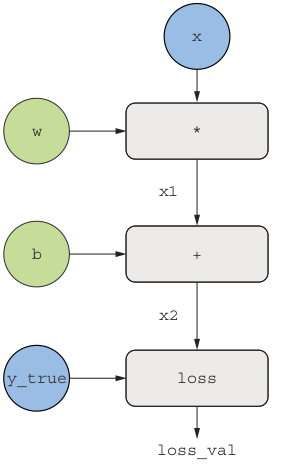
\includegraphics[scale=0.5]{figuras/grafo_computacional.png}
    \caption{Grafo computacional}
\end{figure}

Sabendo que cada uma das duas rodas sequem as equações:
\begin{align}
    \frac{1}{r}
    \begin{bmatrix}
        \sin(\alpha + \beta) &  -\cos(\alpha + \beta) & -l\cos(\beta) \
    \end{bmatrix}
    \dot{\xi}
    = \phi \\
    \begin{bmatrix}
        \cos(\alpha + \beta) &  \sin(\alpha + \beta) & l\sin(\beta) \
    \end{bmatrix}
    \dot{\xi}
    = 0 
\end{align}
Através dessa estrutura de dados e das equações, foi
modelado os parâmetros de uma rede neural artificial,
onde $\alpha$,$\beta$,$r$,$l$ são seus parâmetros,
$\dot{\xi}$ a entrada do modelo e $\phi$ e $0$  são a saídas desejadas.
O grafo computacional com essas operações são representadas por essas equações:

\begin{align}
    \gamma = \alpha + \beta \\
    \cos_{\gamma} = \cos(\gamma) \\
    \sin_{\gamma} = \sin(\gamma) \\
    l_{\phi} = \frac{-l\cos(\beta)}{r} \\
    l_{0} = l\sin(\beta) \\
    W_{\phi_1} = \frac{\sin_{\gamma}}{r} \\
    W_{\phi_2} = \frac{-\cos_{\gamma}}{r} \\
    W_{\phi} = \textbf{tensor\_concat\_h}(_{\phi_1},_{\phi_2}, l_{\phi})\\
    W_{0} = \textbf{tensor\_concat\_h}(\cos_{\gamma},\sin_{\gamma},  l_{0}) \\
    W = \textbf{tensor\_concat\_v}( W_{\phi}, W_{0} ) \\
    y_{\textbf{pred}} =  W \times  \dot{\xi} 
\end{align}
onde cada variável é um tensor, e a
função \textbf{tensor\_concat\_h} junta os tensores horizontalmente:
\begin{align}
    \alpha = 
    \begin{bmatrix}
         \alpha_{1,1} \\
         \alpha_{2,1}
    \end{bmatrix}
    \\
    \beta =
    \begin{bmatrix}
        \beta_{1,1} \\
        \beta_{2,1}
   \end{bmatrix}\\
   \textbf{tensor\_concat\_h}( \alpha, \beta ) =
   \begin{bmatrix}
    \alpha_{1,1} && \beta_{1,1} \\
    \alpha_{2,1} &&  \beta_{2,1} \\
\end{bmatrix}
\end{align}
e \textbf{tensor\_concat\_v} junta os tensores verticalmente:
\begin{align}
    \alpha = 
    \begin{bmatrix}
         \alpha_{1,1} \\
         \alpha_{2,1}
    \end{bmatrix}
    \\
    \beta =
    \begin{bmatrix}
        \beta_{1,1} \\
        \beta_{2,1}
   \end{bmatrix}\\
   \textbf{tensor\_concat\_v}( \alpha, \beta ) =
   \begin{bmatrix}
    \alpha_{1,1} \\
    \alpha_{2,1} \\
    \beta_{1,1} \\
    \beta_{2,1} \\
\end{bmatrix}
\end{align}
Perceba que $W_{\phi}$ representa as equações das rodas, onde
o valor desejado são as velocidades angulares $\phi_1,\phi_2$ das rodas:

\begin{align}
    W_{\phi} = 
    \begin{bmatrix}
        \frac{\sin(\alpha_{1,1} + \beta_{1,1})}{r_1} &  \frac{-\cos(\alpha_{1,2} + \beta_{1,2})}{r_1} & \frac{-l\cos(\beta_{1,3})}{r_1} \\
        \frac{\sin(\alpha_{2,1} + \beta_{2,1})}{r_2} &  \frac{-\cos(\alpha_{2,2} + \beta_{2,2})}{r_2} & \frac{-l\cos(\beta_{2,3})}{r_2}
    \end{bmatrix}
\end{align}

Na prática estamos fazendo uma regressão não linear para encontrar
os parâmetros de uma transformação linear, então podemos também pensar em
grafo de computacional mais simples semelhante a
figura \ref{fig:grafo:computacional} mas sem o parâmetros $b$, 
que encontra a melhor transformação
linear que satisfaça o conjunto de dados coletados,
Neste caso podemos modelar o grafo de maneira mais simples: $\phi=W \times \dot{\xi}$,
onde cada peso é $W_{i,j}$ é encontrado separadamente. Ambos os modelos foram
treinados e foram discutidos na sessão de experimentos e resultados.


\section{pre-processamento dos dados}
A coleta de dados nos fornece dados de posição, orientação, velocidade angular
das rodas do robô e tempo de simulação, portanto temos que transformar os dados
de posição e orientação e tempo, em informação de velocidade linear e angular
do robô, sendo que a velocidade linear tem que está no referencial do robô. O
O pseudo código do pre-processamento pode ser observado no Algoritmo \ref{pre:processamento:}

\begin{algorithm}[H]
    \label{pre:processamento:}
    
    \Entrada{$F$:arquivo resultante da coleta de dados }
    %% \SetLine
    
    $(x_1,y_1,\theta_{1},t_1,\phi_l,\phi_r),(x_2,y_2,\theta_{2},t_2) \leftarrow$ leitura da coleta dados dos instantes de
    tempo $t_1$ e $t_2$

    $\Delta x \leftarrow x_2 - x_1$
    
    $\Delta y \leftarrow y_2 - y_1$

    $\Delta t \leftarrow t_2 - t_1$

    $\Delta \theta \leftarrow \theta_2 - \theta_1$

    \Se {$\Delta \theta > \pi$ }{
                $\Delta \theta \leftarrow \Delta \theta -2\pi $
    }

    \Se {$\Delta \theta < -\pi$ }{
                $\Delta \theta \leftarrow \Delta \theta +2\pi $
    }

    $\text{vel}_{\text{linear}_G} \leftarrow \frac{(\Delta x,\Delta y)}{\Delta t}$

    $\text{vel}_{\text{angular}} \leftarrow \frac{\Delta \theta}{\Delta t}$



    \Para {$i \leftarrow 0$ \Ate $N_a$} {
       
        $
        R(\theta) \leftarrow 
        \begin{bmatrix}
            cos(\theta_{1,i})  & sin(\theta_{1,i})\\
            -sin(\theta_{1,i}) & cos(\theta_{1,i})\\
        \end{bmatrix}
        $

        $\text{vel}_{\text{linear}_{R,i}} \leftarrow R(\theta) \times \text{vel}_{\text{linear}_{G,i}}$
    }
    
    entrada\_modelo\_cinemático $\leftarrow (\text{vel}_{\text{linear}_{R}},\text{vel}_{\text{angular}})$

    
    \eSe {for a entrada do modelo simples: $\phi=W \times \dot{\xi}$}{
                    
        saída\_modelo\_cinemático $\leftarrow (\phi_l,\phi_r)$
      }
      {
        saída\_modelo\_cinemático $\leftarrow (\phi_l,\phi_r,0,0)$
      }

   

      \Retorna entrada\_modelo\_cinemático, saída\_modelo\_cinemático
    
    \caption{Pre-processamento dos dados}
    
\end{algorithm}

Perceba que após a leita dos dados entrada é feita uma aproximação da
velocidade angular e linear do robô através das variação de deslocamento
sobre variação de tempo, também ao calcular a variação da orientação do robô
é verificado se a diferença angular resultante $\Delta \theta$ é a menor.
 É importante salientar que $N_a$
é um número de amostras coletadas, este número pode ser recuperado através
do tamanho de um dos vetores: $x_1,y_1,\theta_{1},t_1,\phi_l,\phi_r,x_2,y_2,\theta_{2},t_2$.
Como dito anteriormente, foram testados dois modelos, um modelo mais complexo
que envolve modelagem dos parâmetros da rede através das equações das rodas
e outro modelo mais simples que busca encontrar uma transformação linear
para os conjunto de dados, quando é realizado o treinamento do modelo complexo
é adicionado mais dois vetores de zeros a saída do modelo cinemático, zeros
que são esperados pelas equações das rodas. 